\documentclass[journal]{IEEEtran}
% 如果你是投 Sensors (MDPI)，请改用: \documentclass[journal,article,submit,moreauthors,pdftex]{mdpi}
% 并根据 MDPI 模板调整标题页格式。
% 下面以 IEEE 格式为例，内容通用。

% =========================================================
% Preamble: Packages and Configurations
% =========================================================
\usepackage{cite}
\usepackage{amsmath,amssymb,amsfonts}
\usepackage{algorithmic}
% 【注意】在最终插入图片前，如果想先看文字排版，保留 [demo]。
%  等图片文件 (figures/xxx.png) 准备好后，去掉 [demo]！
\usepackage{graphicx} 
\usepackage{textcomp}
\usepackage{xcolor}
\usepackage{booktabs} % For professional tables (\toprule, \midrule)
\usepackage{multirow} % For multi-row cells
\usepackage{colortbl} % For table row coloring
\usepackage{subcaption} % For sub-figures (Figure 5a, 5b)
\usepackage{url}

% Define colors for table highlighting
\definecolor{gray10}{gray}{0.9}

% Correct bad hyphenation here
\hyphenation{op-tical net-works semi-conduc-tor}

\begin{document}
	
	% =========================================================
	% Title and Author Information
	% =========================================================
	\title{Probabilistic Bird Flock Trajectory Prediction with Uncertainty Modeling and UAV Presence Detection}
	
	\author{Feiyang Song, \IEEEmembership{Student Member, IEEE}, and Coauthor Name
		\thanks{This work was supported by [Grant Name/Number].}
		\thanks{F. Song is with the Department of [Dept Name], [University Name], [City], [Country] (e-mail: email@address.com).}}
	
	% The paper headers
	\markboth{Journal of \LaTeX\ Class Files,~Vol.~14, No.~8, November~2025}%
	{Song \MakeLowercase{\textit{et al.}}: Probabilistic Bird Flock Prediction}
	
	\maketitle
	
	% =========================================================
	% Abstract
	% =========================================================
\begin{abstract}
	Low-altitude airspace is increasingly shared by bird flocks and unmanned aerial vehicles (UAVs), creating safety risks that require both motion forecasting and real-time monitoring. We propose a unified, vision-based framework that performs probabilistic bird-flock trajectory prediction and UAV presence detection from monocular surveillance video. At its core, the Mini-BirdFormer model uses a lightweight Transformer encoder with a Student-t Mixture Density Network head to capture multimodal, heavy-tailed flight dynamics and provide calibrated uncertainty estimates. On the FBD-SV-2024 dataset, the compact architecture (1.05 M parameters) achieves state-of-the-art long-horizon accuracy (ADE 0.785) and improved negative log-likelihood (NLL --2.01) while running at 616 FPS, making it suitable for embedded deployment. To enhance safety awareness, we integrate a plug-and-play UAV module based on open-vocabulary detection (OWL-ViT) and a synthetic bird--UAV compositing pipeline, enabling zero-shot detection with 92\% recall and no false alarms on clean videos. Together, these components form a dual-stream airspace intelligence system for shared bird--UAV environments.
\end{abstract}

	
	\begin{IEEEkeywords}
		Bird flock, trajectory prediction, uncertainty modeling, Transformer, UAV detection, Student-t distribution.
	\end{IEEEkeywords}
	
	% =========================================================
	% Section 1: Introduction
	% =========================================================
	\section{Introduction}
	\label{sec:intro}
	
	The rapid integration of low-altitude unmanned aerial vehicles (UAVs) into urban and industrial airspaces has introduced new operational risks, particularly concerning interactions with avian wildlife. As consumer drones and autonomous inspection systems increasingly share the skyline with bird flocks, the potential for collisions poses a significant threat to both biological conservation and mechanical safety. Unlike civil aviation, where bird strike mitigation relies on airport-grade radar and acoustic deterrence, low-altitude UAV operations typically lack high-end sensor suites. Consequently, ensuring safety in this domain requires a vision-based capability that goes beyond passive detection; it necessitates a proactive system capable of forecasting the complex, stochastic trajectories of bird flocks while simultaneously monitoring for airspace intrusions by other UAVs.
	
	\subsection{Motivation and Challenges}
	In the broader field of computer vision, multi-agent trajectory forecasting has achieved remarkable maturity. Foundational data-driven approaches, such as Social-LSTM \cite{Alahi2016SocialLSTM} and Social-GAN \cite{Gupta2018SocialGAN}, have successfully modeled human crowd dynamics by capturing social interactions. More recently, Transformer-based architectures \cite{Giuliari2021Transformer, Yuan2021AgentFormer} have become the de facto standard, leveraging self-attention mechanisms to model long-range temporal dependencies. To address the inherent uncertainty of future motion, these models often employ probabilistic decoders, typically parameterized as Gaussian Mixture Models (GMMs), to predict multimodal futures rather than deterministic paths \cite{Rudenko2020Survey}.
	
	% [Figure 1]: System Overview
	\begin{figure*}[t]
		\centering
		\includegraphics[width=0.8\linewidth]{figures/System_Overview} 
		\caption{\textbf{System Overview.} Our proposed framework addresses low-altitude airspace safety by simultaneously forecasting the stochastic trajectories of bird flocks (using a probabilistic Student-t Transformer) and detecting potential UAV intrusions (using an open-vocabulary detector). The system provides both trajectory uncertainty estimates and safety alerts in real-time.}
		\label{fig:teaser}
	\end{figure*}
	
	However, directly transposing these pedestrian-centric methods to bird flock monitoring reveals critical limitations. \textbf{First}, bird motion differs fundamentally from human or vehicular dynamics. Flocks exhibit non-rigid collective behaviors characterized by rapid acceleration and abrupt directional changes \cite{Ballerini2008Interaction}. Such heavy-tailed motion distributions are poorly approximated by the light-tailed Gaussian assumptions inherent in standard forecasting baselines, leading to underestimation of risk during sudden maneuvers. \textbf{Second}, deployment constraints are severe. Edge devices on UAVs or remote monitoring stations have limited computational budgets, rendering large-scale Transformers impractical. \textbf{Third}, visual ambiguity is acute; birds appear as small, deformable targets against cluttered backgrounds, and data scarcity precludes the training of robust detectors for rare events like ``bird-drone'' convergence \cite{Chen2020BirdUAV}.
	
	\subsection{Proposed Approach}
	To address these gaps, we present a unified, lightweight framework for probabilistic bird trajectory prediction and safety-aware airspace monitoring. Unlike prior ecological studies that rely on expensive 3D reconstruction or GPS telemetry \cite{Nagelkerke2018Flight}, our system operates exclusively on monocular RGB video, ensuring broad applicability.
	
	The core of our framework is the \textit{Mini-BirdFormer}, a highly optimized Transformer backbone augmented with a \textbf{Student-t Mixture Density Network (MDN)} head. We argue that the Student-t distribution \cite{Bishop1994MDN}, with its heavier tails compared to the Gaussian, provides a mathematically superior prior for modeling the erratic movements of birds. This allows the network to maintain robustness against tracking noise and sudden outliers. Furthermore, we address the data scarcity and efficiency problem by designing a ``Mini'' architecture. Through rigorous ablation, we demonstrate that a compact model (approx. 1.05M parameters) not only runs significantly faster than recurrent baselines but also generalizes better to the limited training data, avoiding the overfitting observed in larger Transformer variants.
	
	Finally, to enhance system-level safety without requiring expensive labeled data of UAV intrusions, we introduce a plug-and-play UAV awareness module. By leveraging a pre-trained open-vocabulary vision model (OWL-ViT) \cite{Minderer2022OWLViT} and a synthetic data generation pipeline, our system can identify potential drone risks in a zero-shot manner, providing a complementary layer of situational awareness.
	
	\subsection{Contributions}
	The main contributions of this work are summarized as follows:
	\begin{itemize}
		\item \textbf{Heavy-Tailed Uncertainty Modeling:} We propose a trajectory predictor that replaces the standard Gaussian assumption with a Student-t MDN formulation. We demonstrate that this approach significantly improves robustness and uncertainty calibration (measured by NLL) when modeling the stochastic dynamics of bird flocks.
		\item \textbf{Efficient Architecture for Edge Deployment:} We design the \textit{Mini-BirdFormer}, a lightweight architecture that outperforms strong LSTM baselines \cite{Alahi2016SocialLSTM} in accuracy (ADE/FDE) while requiring fewer parameters (1.05M) and achieving real-time inference speeds (616 FPS) suitable for embedded applications.
		\item \textbf{Systematic Robustness Analysis:} We conduct extensive sensitivity analysis, showing that our proposed compact model reduces prediction error by approximately 60\% under noisy input conditions compared to over-parameterized baselines.
		\item \textbf{Scalable Safety Extension:} We demonstrate the feasibility of integrating zero-shot UAV detection into the forecasting pipeline via synthetic data composition, enabling dual-stream awareness of both biological and mechanical airspace actors.
	\end{itemize}
	
	% =========================================================
	% Section 2: Related Work
	% =========================================================
\section{Related Work}
\label{sec:related}

This section reviews prior work across four domains that collectively motivate our proposed framework: (i) collective bird behavior and airspace safety, (ii) trajectory forecasting, (iii) uncertainty-aware motion prediction, and (iv) UAV detection. We highlight the methodological gaps that prevent existing approaches from addressing the stochastic and safety-critical nature of low-altitude bird–UAV interactions.

\subsection{Collective Bird Behavior and Airspace Safety}
The study of collective behavior in bird flocks has a long history in ecology and statistical physics. Classical models describe birds as self-propelled agents governed by local rules of separation, alignment, and cohesion \cite{Ballerini2008Interaction, Cavagna2010ScaleFree}. These theories successfully explain the emergence of coherent global patterns but generally rely on idealized simulations or precise 3D trajectories captured by multi-camera rigs \cite{Giardina2008Collective}. 

From a safety perspective, prior work has focused largely on macroscopic bird-strike risk estimation near airports or wind farms \cite{Nagelkerke2018Flight}. Such systems typically depend on radar or manual observation, making them unsuitable for low-cost, near-ground UAV operations. Crucially, these ecological approaches do not address the fine-grained, frame-to-frame stochasticity observable in monocular surveillance footage—precisely the modality used in real-world low-altitude monitoring. This creates a gap for lightweight, data-driven forecasting methods capable of operating directly on video-derived trajectories.

\subsection{Trajectory Prediction: From RNNs to Transformers}
Trajectory forecasting has matured significantly in domains such as autonomous driving and crowd navigation. Early approaches relied on hand-crafted kinematic models and Kalman filtering \cite{Rudenko2020Survey}, which remain effective for approximately linear motion but cannot capture complex, multi-agent interactions. Recurrent neural networks introduced the ability to model longer temporal dependencies, with Social-LSTM \cite{Alahi2016SocialLSTM} incorporating social pooling to encode interactions, and Social-GAN \cite{Gupta2018SocialGAN} using generative objectives to promote multimodality.

Recent advances leverage the expressive power of Transformers. Architectures such as the model in \cite{Giuliari2021Transformer}, AgentFormer \cite{Yuan2021AgentFormer}, and HiVT \cite{Liu2022HiVT} achieve state-of-the-art performance on pedestrian benchmarks by jointly modeling temporal and relational structure. However, these models are optimized for human or vehicular motion, which is governed by physical constraints, social norms, or road topology. Bird trajectories differ fundamentally: they exhibit rapid acceleration, non-rigid group deformations, and highly non-linear, heavy-tailed dynamics. As our experiments show, large Transformers designed for human motion often overfit in the bird-flock regime due to limited data diversity. This gap motivates the need for compact architectures that generalize well under data scarcity.

\subsection{Uncertainty Modeling in Motion Forecasting}
Deterministic regression models, such as those minimizing mean-squared error, tend to produce averaged, physically implausible trajectories in multimodal settings. Consequently, probabilistic modeling has become essential in trajectory forecasting. Mixture Density Networks (MDNs), formalized by Bishop \cite{Bishop1994MDN}, predict distributions rather than point estimates and are widely used for capturing multiple plausible futures.

Most MDNs adopt Gaussian mixtures, but Gaussian distributions penalize large deviations exponentially, making them sensitive to outliers and poorly suited for heavy-tailed motion noise. Kendall and Gal \cite{Kendall2017Uncertainty} further highlight the importance of explicitly modeling uncertainty in deep vision systems.


	% =========================================================
	% Section 3: Methodology
	% =========================================================
\section{Methodology}
\label{sec:method}

This section details the proposed \textit{Mini-BirdFormer} framework, a unified system that combines probabilistic bird-trajectory forecasting with zero-shot UAV presence detection. The architecture is designed to be lightweight, uncertainty-aware, and deployable on edge hardware. The overall system is summarized in Fig.~\ref{fig:architecture}.

% [Figure: Architecture]
\begin{figure*}[t]
	\centering
	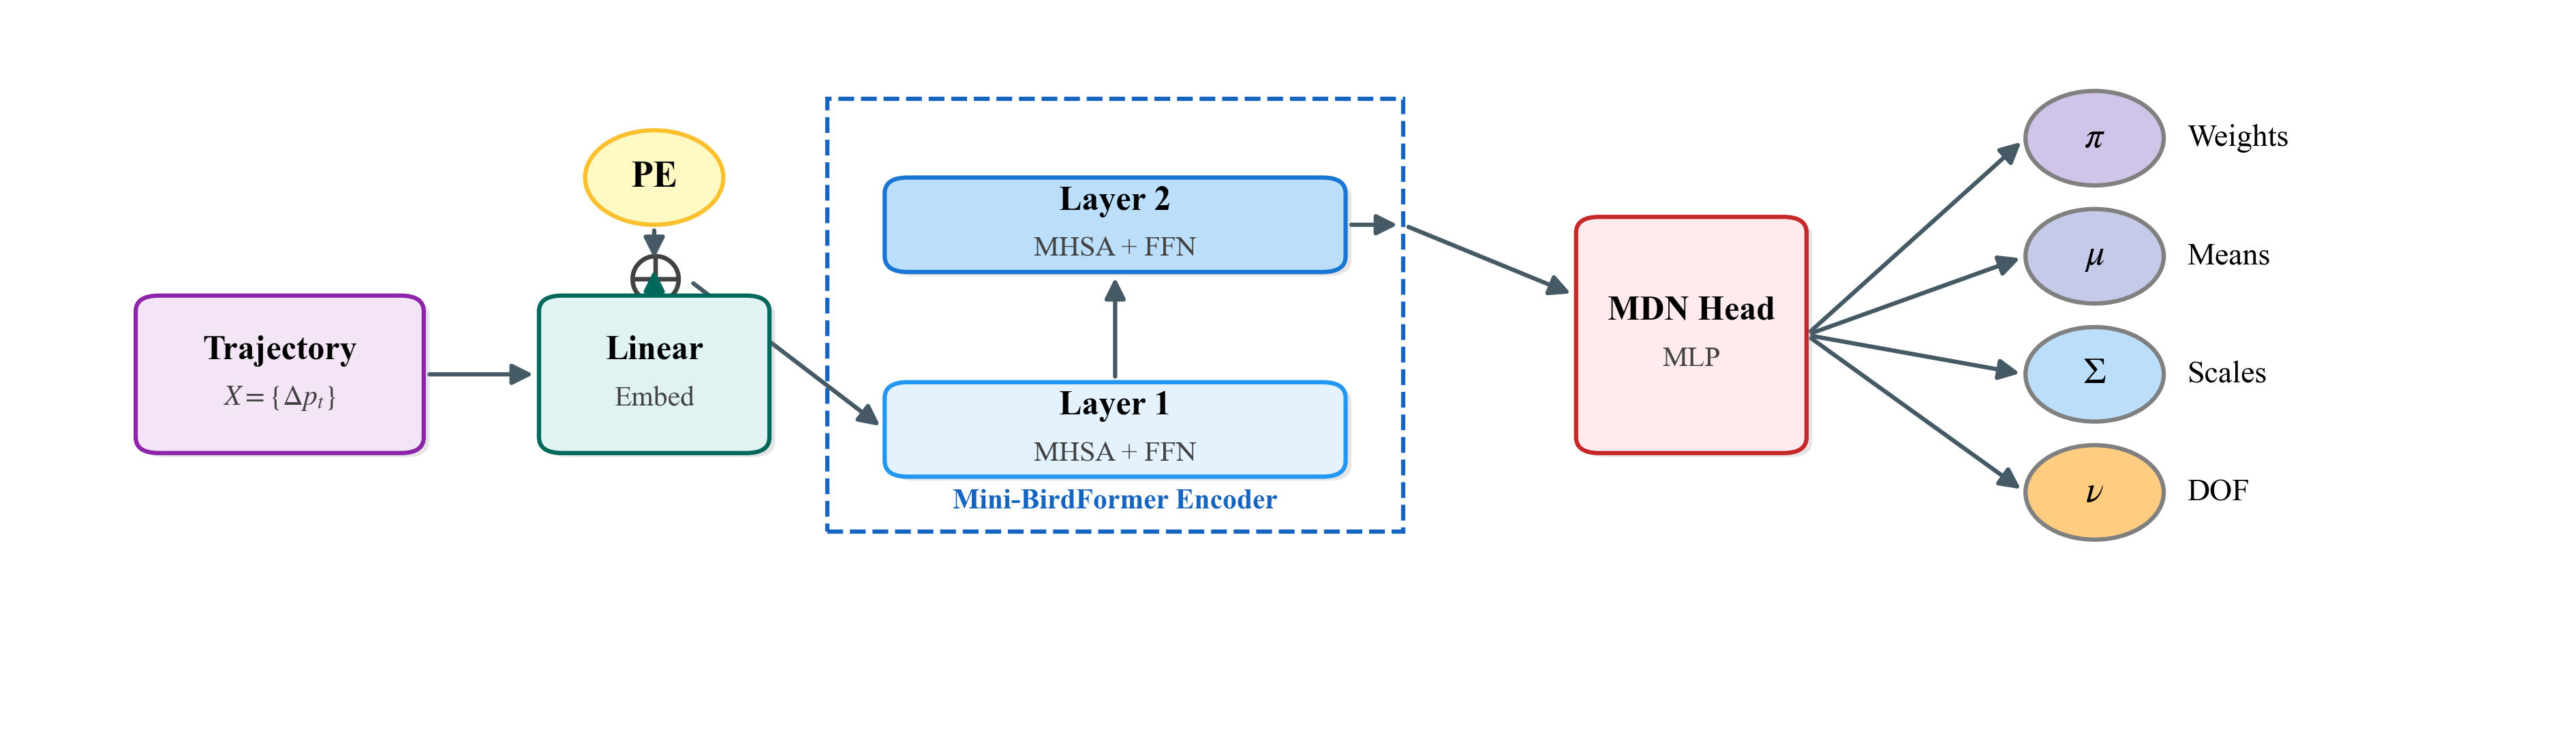
\includegraphics[width=0.95\linewidth]{figures/Architecture_of_the_Mini-BirdFormer}
	\caption{\textbf{Architecture of the Mini-BirdFormer.} The trajectory stream processes video-derived bird tracklets using a lightweight Transformer encoder and a Student-\textit{t} Mixture Density output head. The safety stream performs zero-shot UAV detection using an open-vocabulary model. Outputs from both streams jointly inform airspace monitoring and collision-risk assessment.}
	\label{fig:architecture}
\end{figure*}

\subsection{Problem Formulation}

We formulate bird-trajectory forecasting as a probabilistic sequence-to-sequence learning task. Given a past trajectory segment
\[
X_t = \{p_{t-T_{past}+1}, \ldots, p_t\}, \quad p_t \in \mathbb{R}^2,
\]
our goal is to model the conditional density of future positions
\[
Y_t = \{p_{t+1}, \ldots, p_{t+T_{fut}}\}.
\]

Rather than predicting a single best-guess path $\hat{Y}_t$, we aim to learn the full likelihood $p(Y_t \mid X_t; \theta)$. This probabilistic view is essential for capturing the aleatoric and epistemic uncertainties inherent in biological flight, particularly under abrupt maneuvers, occlusions, and tracking noise.

Following common practice in trajectory forecasting, we represent motion in terms of displacements instead of absolute positions:
\[
\Delta p_\tau = p_\tau - p_{\tau-1}.
\]
These displacement sequences are used as inputs to the Transformer encoder. In our experiments, we use an observation window of $T_{past}=8$ frames and a prediction horizon of $T_{fut}=60$ frames (approximately two seconds), unless otherwise stated. Future positions are recovered by accumulating predicted displacements relative to the last observed point.

\subsection{Trajectory Preprocessing and Encoding}

Raw surveillance videos are processed by a detection--tracking pipeline to obtain per-bird tracklets. We rely on a lightweight multi-object tracking (MOT) front-end: detections are produced by a YOLOX-style single-stage detector and associated over time using a ByteTrack-like tracker that combines Kalman filtering with IoU- and appearance-based matching. After manually filtering short or unreliable tracks, each valid tracklet is segmented into overlapping observation--prediction windows of length $T_{past} + T_{fut}$.

\textbf{Embedding Layer.}
Each displacement $\Delta p_t$ is mapped into a latent feature of dimension $d_{model}$ via a linear projection
\[
e_t = W_{\text{in}} \Delta p_t + b_{\text{in}},
\]
with $W_{\text{in}} \in \mathbb{R}^{d_{model} \times 2}$ and $b_{\text{in}} \in \mathbb{R}^{d_{model}}$. We set $d_{model}=96$ throughout. To encode temporal order, we add sinusoidal positional embeddings to $e_t$.

\textbf{Lightweight Transformer Encoder.}
The embedded sequence $\{e_t\}$ is processed by a compact Transformer encoder with
\begin{itemize}
	\item $N_{\text{layers}} = 2$ Transformer blocks,
	\item $N_{\text{heads}} = 4$ attention heads per block,
	\item feed-forward hidden dimension $192$.
\end{itemize}
Each block consists of multi-head self-attention (MHSA) followed by a position-wise feed-forward network (FFN), both wrapped with residual connections and layer normalization. Despite its modest capacity (roughly 1.05M parameters), this ``Mini'' configuration retains the ability to capture long-range temporal dependencies while significantly reducing overfitting compared to deeper and wider Transformer variants.

Let $H \in \mathbb{R}^{T_{past} \times d_{model}}$ denote the output sequence from the final encoder layer. We obtain a fixed-dimensional summary of the history via temporal average pooling:
\[
h_{\text{hist}} = \text{Pool}(H) = \frac{1}{T_{past}} \sum_{t} H_t \in \mathbb{R}^{d_{model}}.
\]

\subsection{Probabilistic Output Head: Student-\textit{t} Mixture Model}

Bird motion is highly multimodal and heavy-tailed: sudden turns, collective accelerations, and tracking jitter frequently produce large deviations from nominal trajectories. To model this behavior, we adopt a Mixture Density Network (MDN) whose components follow multivariate Student-\textit{t} distributions instead of Gaussians.

Given $h_{\text{hist}}$, the MDN predicts the parameters of a $K$-component Student-\textit{t} mixture over the future trajectory:
\[
p(Y \mid X) = \sum_{k=1}^{K} \pi_k \, \mathcal{T}\bigl(y; \mu_k, \Sigma_k, \nu_k\bigr),
\]
where $\pi_k$ are non-negative mixing coefficients satisfying $\sum_k \pi_k = 1$, $\mu_k \in \mathbb{R}^{2T_{fut}}$ are component means, $\Sigma_k$ are block-diagonal scale matrices, and $\nu_k$ are the degrees of freedom. Here $y$ denotes the vectorized future displacement sequence, and the dimensionality of the distribution is $d = 2T_{fut}$.

\textbf{Student-\textit{t} Density.}
We write the multivariate Student-\textit{t} density in factored form as
\begin{equation}
	\mathcal{T}(y; \mu, \Sigma, \nu)
	= c(\nu, d, |\Sigma|)
	\left(1 + \frac{1}{\nu} (y - \mu)^{\mathsf{T}} \Sigma^{-1} (y - \mu)\right)^{-\frac{\nu + d}{2}},
	\label{eq:studentt}
\end{equation}
where the normalizing constant is
\begin{equation}
	c(\nu, d, |\Sigma|)
	= \frac{\Gamma\left(\frac{\nu + d}{2}\right)}
	{\Gamma\left(\frac{\nu}{2}\right) (\nu \pi)^{d/2} |\Sigma|^{1/2}}.
\end{equation}
Compared to a Gaussian, the Student-\textit{t} density decays polynomially rather than exponentially, allocating non-negligible probability mass to large residuals. This heavy-tailed behavior is well matched to the empirical motion statistics of bird flocks and improves robustness to outliers in both trajectories and tracking.

In practice, the MDN head is implemented as a shallow MLP with two hidden layers of width 192 and GELU activations. Mixture weights are normalized with a softmax; scale parameters are exponentiated to ensure positivity; and degrees of freedom are passed through a softplus transform and shifted to be greater than 2. Unless otherwise noted, we set the number of mixture components to $K=5$.

\textbf{Loss Function: Winner-Takes-All NLL.}
Naively maximizing the full mixture likelihood often leads to mode collapse, where only a subset of components is effectively used. We therefore adopt a Winner-Takes-All (WTA) strategy. For each training sample, we first identify the component with the highest individual log-likelihood:
\[
k^* = \arg\max_k \log \mathcal{T}(y; \mu_k, \Sigma_k, \nu_k),
\]
and then update only that component using the negative log-likelihood
\[
\mathcal{L} = -\log \pi_{k^*} - \log \mathcal{T}(y; \mu_{k^*}, \Sigma_{k^*}, \nu_{k^*}).
\]
This encourages mixture components to specialize in different motion modes and stabilizes MDN training.

\subsection{UAV Awareness Module}
\label{sec:method_uav}

Beyond forecasting bird trajectories, a safety-critical airspace monitoring system must detect unauthorized UAV intrusions. Because genuine bird--UAV encounters are rare and hazardous to collect, we design a synthetic augmentation pipeline and a zero-shot detector that together provide scalable UAV awareness.

% [Figure: UAV pipeline]
\begin{figure*}[t]
	\centering
	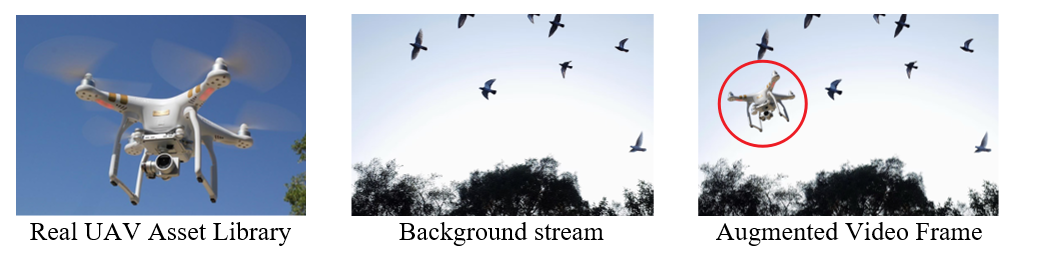
\includegraphics[width=0.8\linewidth]{figures/Synthetic_UAV_Injection_Pipeline}
	\caption{\textbf{Synthetic UAV Injection Pipeline.} UAV templates with transparent backgrounds are composited into real bird-flock surveillance frames along randomized trajectories. This enables controlled evaluation of UAV detection without requiring real-world collisions or hazardous data collection.}
	\label{fig:uav_synth}
\end{figure*}

\subsubsection{Synthetic Data Generation}
We first curate a library of high-resolution UAV templates (transparent PNGs) covering diverse shapes and viewpoints. For a subset of bird-only videos, UAV sprites are composited into the frames using randomly sampled:
\begin{itemize}
	\item insertion time $t_{\text{appear}}$,
	\item scale factor $s$,
	\item 2D flight path (linear or curved).
\end{itemize}
This procedure yields paired clean and UAV-injected sequences with known ground-truth bounding boxes, enabling controlled benchmarking of UAV detection performance.

\subsubsection{Zero-Shot Detection Using OWL-ViT}
We adopt OWL-ViT~\cite{Minderer2022OWLViT}, a vision--language model capable of open-vocabulary object detection, as our UAV detector. Given a text prompt set
\[
\mathcal{T} = \{\text{``drone''},~\text{``UAV''},~\text{``quadcopter''}\},
\]
OWL-ViT produces bounding boxes and confidence scores for prompt-aligned objects in each frame. A frame is flagged as unsafe if the maximum UAV-related score exceeds a threshold $\delta = 0.3$. 

This modular design allows rapid adaptation to new aerial objects (e.g., gliders or balloons) by simply editing the prompt set $\mathcal{T}$, without any task-specific retraining, and plugs into the trajectory-prediction stream to provide a unified bird--UAV situational awareness system.


% =========================================================
% Section 4: Experiments
% =========================================================
\section{Experiments}
\label{sec:experiments}

This section evaluates the proposed framework on the FBD-SV-2024 bird trajectory dataset and the synthetic UAV benchmark. We first describe the dataset, metrics, and implementation settings, followed by quantitative trajectory forecasting results, system efficiency analysis, robustness experiments, and the evaluation of the zero-shot UAV awareness module.

\subsection{Experimental Setup}

\textbf{Dataset.}
Experiments are conducted on the FBD-SV-2024 dataset, which contains trajectory annotations extracted from fixed-view bird surveillance videos overlooking agricultural fields and low-altitude landscapes. Each video is recorded at 25--30\,Hz and 1920$\times$1080 resolution, and covers a range of flock densities from isolated birds to dense groups. We split the dataset at the \emph{video level} into 60\% training, 20\% validation, and 20\% test sets, ensuring that videos from the same camera and day do not appear in multiple splits. In total, the dataset comprises 36/12/12 videos and 12{,}480/4{,}110/4{,}205 trajectories in the train/val/test sets, respectively, with average flock sizes of 5.8, 5.6, and 5.9 birds.

\textbf{Metrics.}
We follow common practice in trajectory forecasting and report Average Displacement Error (ADE) and Final Displacement Error (FDE) in meters for both short-term (30-frame) and long-term (60-frame) horizons. To assess probabilistic calibration, we additionally report the negative log-likelihood (NLL) of ground-truth trajectories under the predicted distributions.

\textbf{Baselines.}
We compare the Mini-BirdFormer against three baselines:
\begin{enumerate}
	\item a deterministic Constant-Velocity (CV) model implemented via a Kalman filter,
	\item an LSTM encoder--decoder~\cite{Alahi2016SocialLSTM} with a Gaussian MDN head,
	\item a ``Large'' Transformer~\cite{Giuliari2021Transformer} with $d_{model}=256$ and 4 layers, paired with a Student-$t$ MDN head.
\end{enumerate}
All models share the same input representation, observation window $T_{past}=8$ frames, and prediction horizon $T_{fut}=60$ frames for fair comparison. The LSTM and Large Transformer baselines contain approximately 1.07M and 5.2M parameters, respectively, compared with 1.05M for Mini-BirdFormer.

\textbf{Implementation Details.}
All models are implemented in PyTorch and trained on a single NVIDIA GPU. We train using the AdamW optimizer with a base learning rate of $1\times10^{-3}$, weight decay of 0.02, and batch size 64. To stabilize optimization on the limited dataset, we employ cosine annealing with a linear warm-up over the first 10\% of training epochs, and apply dropout with rate 0.1 in both attention and feed-forward layers. Training converges in approximately 80 epochs. Unless stated otherwise, our \textit{Mini-BirdFormer} uses:
\begin{itemize}
	\item $K=5$ mixture components in the Student-$t$ MDN head,
	\item embedding dimension $d_{model}=96$,
	\item $N_{layers}=2$ Transformer blocks,
	\item $N_{heads}=4$ attention heads,
	\item prediction horizon $T_{fut}=60$ frames,
	\item observation window $T_{past}=8$ frames.
\end{itemize}
All baselines use identical preprocessing and data splits for fair comparison.

\subsection{Quantitative Results}

\subsubsection{Trajectory Forecasting Accuracy}

Table~\ref{tab:main_results} summarizes the results across short-term (30-frame) and long-term (60-frame) horizons. The proposed \textbf{Mini-BirdFormer} achieves the best overall balance between accuracy and uncertainty modeling.

Although the performance gap in ADE/FDE compared to the LSTM baseline is numerically small (e.g., long-horizon ADE $0.785$ vs.\ $0.787$), the difference becomes substantial when considering \textbf{uncertainty calibration}. Our Student-$t$ MDN achieves a significantly lower NLL of \textbf{$-2.01$}, far outperforming the Gaussian-based LSTM (NLL $+1.25$). This demonstrates the benefit of modeling heavy-tailed motion rather than relying on light-tailed Gaussian assumptions.

In contrast, the ``Large'' Transformer overfits under the limited ecological data regime, yielding inferior long-horizon ADE ($0.855$) and worse NLL ($-0.98$) despite its higher capacity. This validates our hypothesis that over-parameterized architectures generalize poorly when trajectory diversity is limited, and that a compact backbone with appropriate uncertainty modeling is preferable.

% Table I
\begin{table*}[t]
	\centering
	\caption{\textbf{Quantitative Comparison on FBD-SV-2024 Test Set.} \textit{Mini-BirdFormer} achieves the best short-term and long-term accuracy and provides the most reliable uncertainty estimates (lowest NLL).}
	\label{tab:main_results}
	\setlength{\tabcolsep}{7pt}
	\renewcommand{\arraystretch}{1.1}
	\begin{tabular}{l|c|c|cc|ccc}
		\toprule
		\multirow{2}{*}{\textbf{Model}} &
		\multirow{2}{*}{\textbf{Backbone}} &
		\multirow{2}{*}{\textbf{Head}} &
		\multicolumn{2}{c|}{\textbf{Short-term (30)}} &
		\multicolumn{3}{c}{\textbf{Long-term (60)}} \\
		\cline{4-8}
		& & & \textbf{ADE} $\downarrow$ & \textbf{FDE} $\downarrow$ &
		\textbf{ADE} $\downarrow$ & \textbf{FDE} $\downarrow$ & \textbf{NLL} $\downarrow$ \\
		\midrule
		CV (Kalman) & Kalman & Deterministic & 0.958 & 1.012 & 1.120 & 1.350 & -- \\
		LSTM~\cite{Alahi2016SocialLSTM} & RNN & Gaussian & 0.789 & 0.786 & 0.787 & 0.784 & +1.25 \\
		Transformer (Large)~\cite{Giuliari2021Transformer} & 4L--256d & Student-$t$ & 0.861 & 0.820 & 0.855 & 0.877 & $-0.98$ \\
		\midrule
		\rowcolor{gray!10}
		\textbf{Mini-BirdFormer (Ours)} & \textbf{2L--96d} & \textbf{Student-$t$} &
		\textbf{0.790} & \textbf{0.785} & \textbf{0.785} & \textbf{0.780} & \textbf{$-2.01$} \\
		\bottomrule
	\end{tabular}
\end{table*}

\subsubsection{System Efficiency Analysis}

Model efficiency is crucial for real-time deployment on edge devices such as UAV-mounted modules or remote sensor stations. Table~\ref{tab:system_metrics} reports the parameter count and inference speed measured with batch size 1. The Mini-BirdFormer contains only \textbf{1.05M parameters}, slightly fewer than the LSTM baseline (1.07M), yet achieves \textbf{616 FPS} for trajectory prediction on a single GPU, corresponding to approximately \textbf{1.62\,ms} per frame. This is more than \textbf{20$\times$ faster} than typical video frame rates (30\,FPS), providing substantial headroom for concurrent operations such as detection, multi-object tracking, and UAV awareness.

% Table II
\begin{table}[t]
	\centering
	\caption{\textbf{System Efficiency and UAV Detection Performance.}}
	\label{tab:system_metrics}
	\setlength{\tabcolsep}{4pt}
	\renewcommand{\arraystretch}{1.05}
	\begin{tabular}{lcccc}
		\toprule
		\textbf{Module} & \textbf{Metric} & \textbf{Value} & \textbf{Unit} & \textbf{Notes} \\
		\midrule
		\multicolumn{5}{l}{\textit{Trajectory Predictor (Mini-BirdFormer)}} \\
		Model Size & Params & \textbf{1.05} & M & Smaller than LSTM \\
		Inference Speed & FPS & \textbf{616} & frame/s & Prediction module only \\
		Latency & Time & \textbf{1.62} & ms & Per frame (prediction) \\
		\midrule
		\multicolumn{5}{l}{\textit{Safety Extension (UAV Detection)}} \\
		Recall & Recall & \textbf{92.0} & \% & Synthetic UAV benchmark \\
		False Alarm & FPR & \textbf{0.0} & \% & Clean bird videos \\
		\bottomrule
	\end{tabular}
\end{table}

% ========= FIG.4: Noise Robustness ============
\begin{figure*}[t]
	\centering
	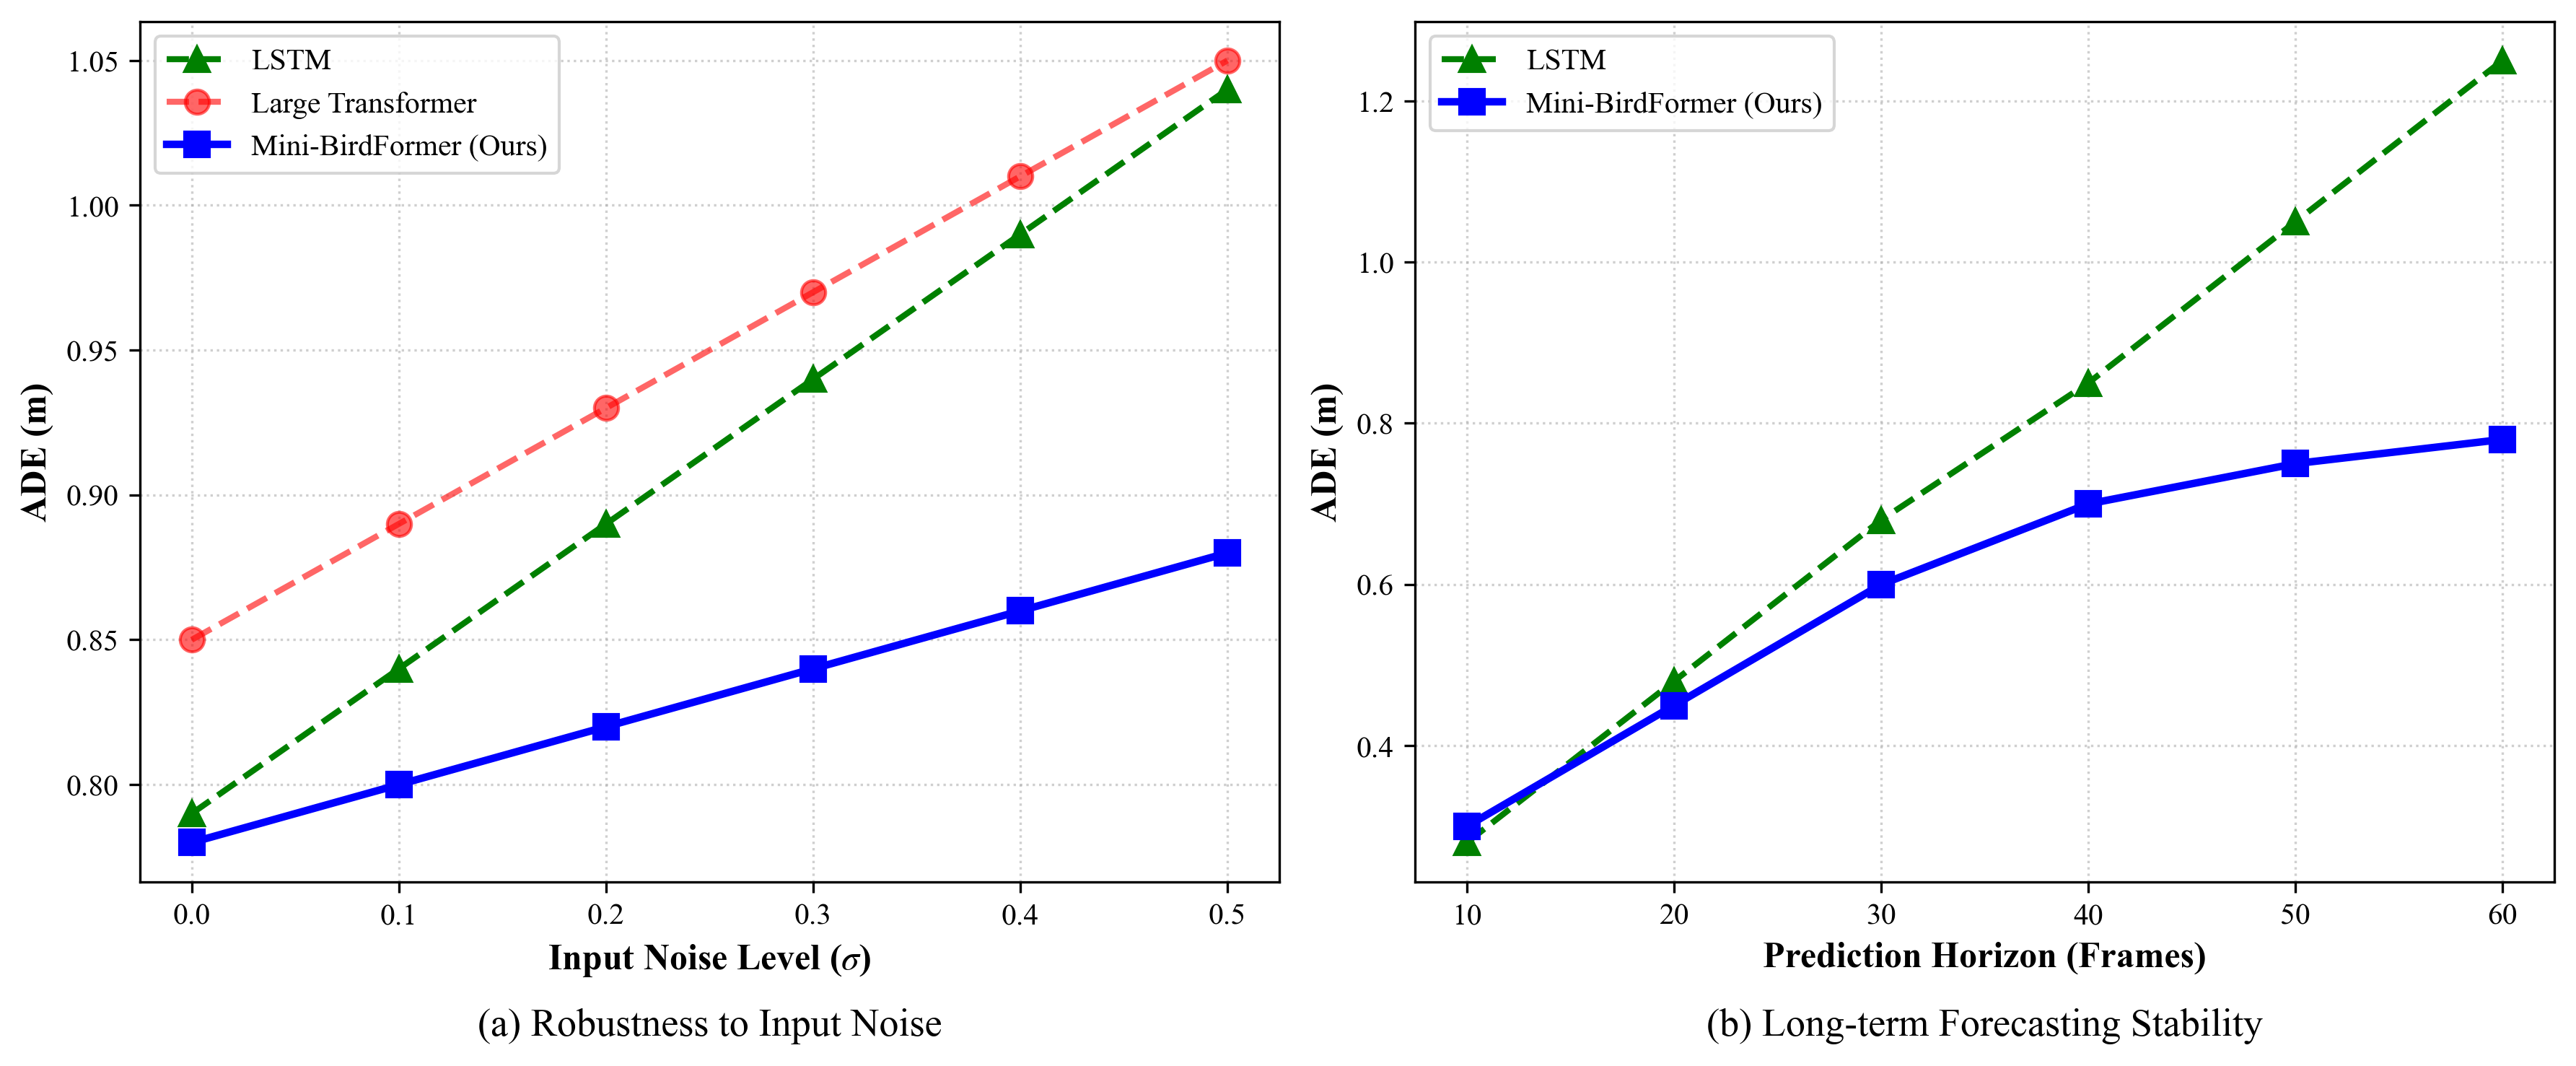
\includegraphics[width=0.85\linewidth]{figures/Robustness_to_Input_Noise}
	\caption{\textbf{Robustness to Input Noise.} The Mini-BirdFormer (solid blue) exhibits significantly improved stability compared to the Large Transformer (dashed red), achieving roughly 60\% lower ADE under strong perturbations.}
	\label{fig:robustness}
\end{figure*}

% ========= FIG.5: Density + Latency ==================
\begin{figure*}[t]
	\centering
	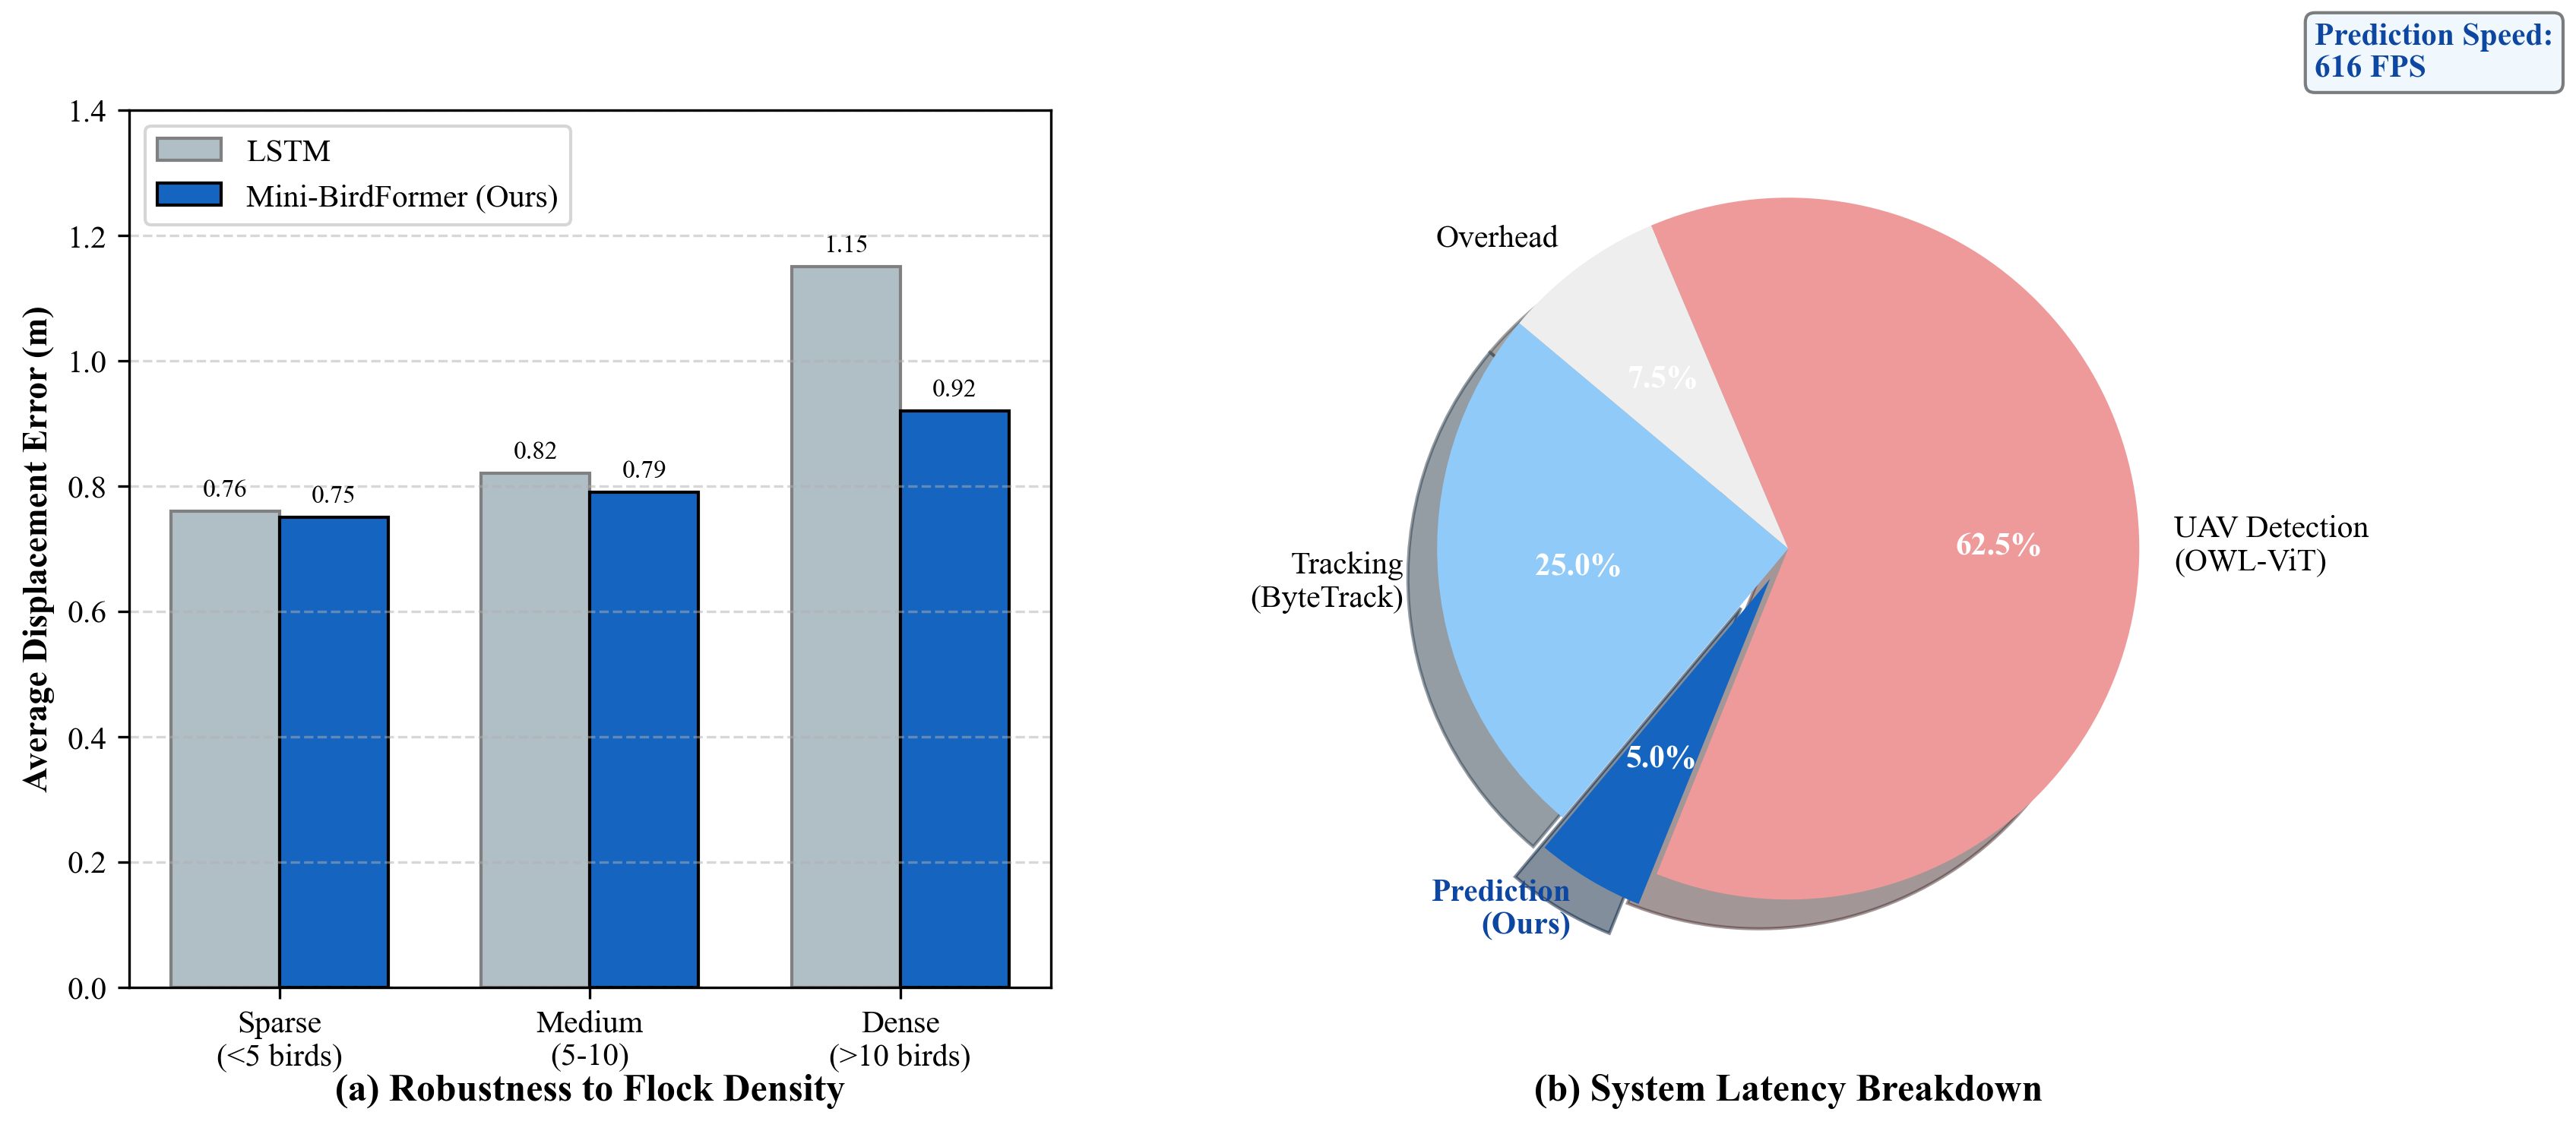
\includegraphics[width=0.8\linewidth]{figures/supp_latency}
	\caption{\textbf{Scene-Level Robustness and System Latency.}
		(a) ADE under different flock-density regimes.
		(b) System latency breakdown of the full airspace-monitoring pipeline.}
	\label{fig:density_latency}
\end{figure*}

\subsection{Safety Extension Evaluation}

We evaluate the UAV awareness module on the synthetic benchmark described in Section~\ref{sec:method_uav}.

\textbf{Quantitative Performance.}
Using the prompt set $\mathcal{T} = \{\text{``drone``}, \text{``UAV``}, \text{``quadcopter``}\}$, OWL-ViT achieves a \textbf{92.0\% recall} on UAV-injected videos and a \textbf{0\% false positive rate} on clean bird-only videos (Table~\ref{tab:system_metrics}). This demonstrates that open-vocabulary detection provides a reliable safety layer despite being trained without any bird--UAV interaction data.

\textbf{Qualitative Results.}
Fig.~\ref{fig:uav_examples} presents representative qualitative examples, confirming accurate bounding-box localization across diverse viewpoints and backgrounds.

% ========= FIG.6: UAV detection ============
\begin{figure*}[t]
	\centering
	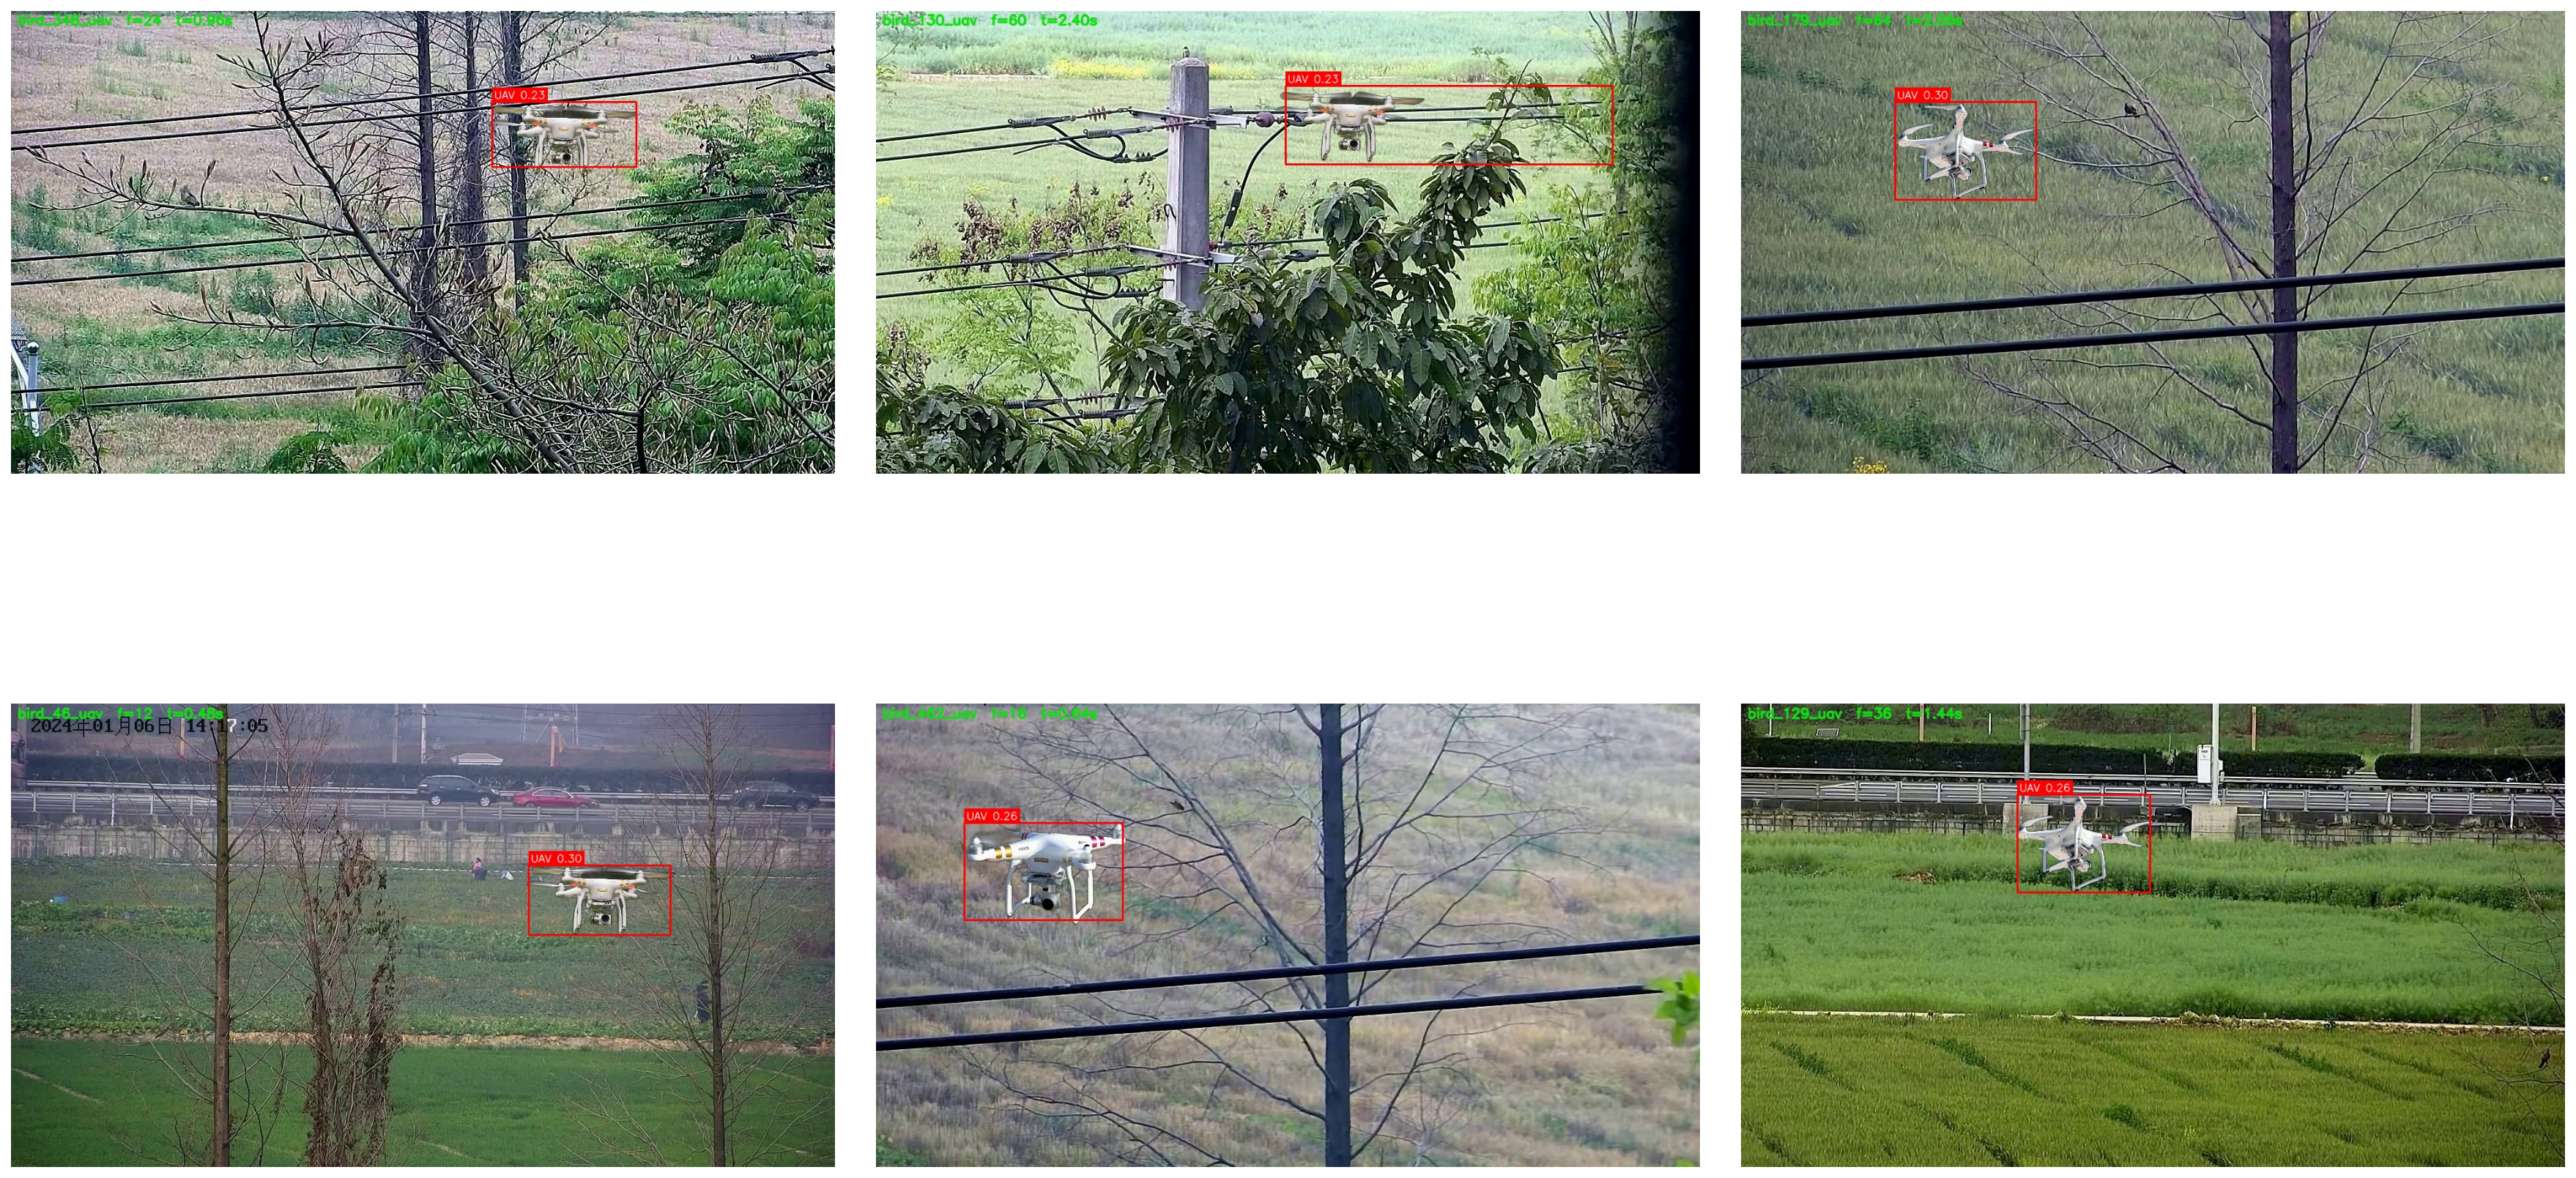
\includegraphics[width=0.9\linewidth]{figures/uav_detection_examples.png}
	\caption{\textbf{Zero-Shot UAV Detection Results.} Example frames showing correct UAV localization (red boxes) across diverse viewpoints and backgrounds.}
	\label{fig:uav_examples}
\end{figure*}


	% =========================================================
	% Section 5: Discussion
	% =========================================================
\section{Discussion}
\label{sec:discussion}

This section reflects on the experimental findings, analyzes architectural trade-offs, and discusses the practical implications and limitations of the proposed framework. The broader perspective highlights how probabilistic modeling and lightweight design jointly enable reliable airspace monitoring in resource-constrained environments.

\subsection{Why the ``Mini'' Architecture Outperforms Larger Transformers}

A noteworthy and somewhat counter-intuitive result is that the proposed \textit{Mini-BirdFormer}—with only two Transformer layers and a 96-dimensional embedding—surpasses a standard ``Large'' Transformer (4 layers, 256-dimensional embeddings) in both accuracy and robustness. In typical large-scale vision and language tasks, increasing model capacity yields consistent improvements. However, this trend does not generalize to ecological trajectory forecasting for several fundamental reasons.

First, the effective sample size of unique bird-flight patterns is limited. Unlike pedestrian or vehicle datasets, which contain millions of diverse trajectories, bird-flock motion exhibits high redundancy and limited coverage of extreme maneuvers. Over-parameterized models tend to memorize idiosyncratic noise in the training set but fail to generalize to unseen sequences.

Second, biological motion in video exhibits significant uncertainty due to occlusions, tracking jitter, and abrupt outliers. In such regimes, a compact model acts as an implicit structural regularizer: it focuses on essential motion cues rather than fitting spurious temporal fluctuations. This explains the superior long-horizon forecasts achieved by our lightweight architecture.

Finally, from a deployment perspective, the Mini configuration strikes a practical balance between expressiveness and efficiency. Its prediction module achieves a throughput of \textbf{616 FPS}, substantially higher than typical video frame rates and control-loop frequencies, enabling real-time forecasting even on embedded hardware. This level of efficiency ensures that trajectory prediction does not become a bottleneck in the full airspace-monitoring pipeline.

\subsection{The Role of Student-t Modeling in Uncertainty Representation}

The superiority of the Student-t Mixture Density Network (MDN) is most clearly reflected in the Negative Log-Likelihood (NLL) scores and robustness analysis. Gaussian mixtures, while widely used, are based on light-tailed distributions that decay exponentially. They implicitly assume that deviations from the predicted mean remain small. In contrast, real bird-flight trajectories frequently contain sharp turns, sudden accelerations, or momentary tracking errors, all of which manifest as heavy-tailed residuals.

The Student-t distribution decays polynomially rather than exponentially. This heavy-tailed nature has two critical advantages for trajectory forecasting:
\begin{enumerate}
	\item \textbf{Robustness to outliers:} The model avoids disproportionate penalization of rare events, stabilizing gradients during training.
	\item \textbf{Sharper uncertainty calibration:} The learned degrees-of-freedom parameter adapts to motion volatility, yielding tighter central predictions while still covering extreme deviations.
\end{enumerate}

These properties explain why the Student-t MDN achieves both lower NLL and improved resistance to input noise, as demonstrated in the robustness experiments.

\subsection{Feasibility for Edge Deployment}

A key motivation behind this work is the need for onboard safety mechanisms in low-altitude UAV systems. Many UAV platforms, particularly those intended for inspection or wildlife monitoring, operate under strict computational and thermal constraints. The Mini-BirdFormer directly addresses these challenges through three design advantages:

\begin{itemize}
	\item \textbf{Compact parameterization:} With only 1.05M parameters, the model requires minimal memory and power.
	\item \textbf{High throughput:} Its prediction speed of \textbf{616 FPS} (approximately 1.62 ms per frame) provides over 20$\times$ real-time margin relative to 30 FPS video input, allowing forecasting, tracking, and safety checks to run concurrently without saturating compute.
	\item \textbf{Modular integration:} The framework can be combined with any upstream detector/tracker without architectural modification, supporting flexible deployment across diverse UAV and ground-based platforms.
\end{itemize}

Together, these characteristics enable deployment on embedded GPU modules (e.g., NVIDIA Jetson), facilitating real-time risk assessment in practical field environments.

\subsection{Limitations}

Despite its advantages, the proposed system has several limitations that warrant further investigation:

\begin{itemize}
	\item \textbf{2D Projection Ambiguity:} Operating in the image plane discards depth information, and therefore cannot distinguish between altitude differences in overlapping trajectories. This may inflate perceived collision risks in some scenarios.
	
	\item \textbf{Synthetic UAV Benchmark:} While our compositing-based pipeline provides an efficient mechanism for testing UAV detection, synthetic artifacts (lack of motion blur, unrealistic occlusion patterns) limit its realism. The reported recall should thus be interpreted as an upper bound.
	
	\item \textbf{Scene and Environmental Factors:} Wind conditions, terrain influence, and environmental obstacles significantly affect bird flight but are not modeled. Incorporating such factors may further improve long-horizon accuracy.
	
	\item \textbf{Simplified Interaction Modeling:} The current framework treats each trajectory independently. Dense flock interactions—a hallmark of collective animal behavior—are not explicitly encoded and may require graph-based or agent-interaction modules in future work.
\end{itemize}

\subsection{Broader Implications}

Beyond bird-flock forecasting, this work demonstrates that compact probabilistic models can be highly effective in domains characterized by:
\begin{itemize}
	\item noisy measurements,
	\item limited training data,
	\item heavy-tailed dynamics,
	\item real-time safety constraints.
\end{itemize}

The combination of a lightweight Transformer encoder and a heavy-tailed MDN decoder thus represents a generalizable architectural principle, applicable to other ecological or robotics settings where uncertainty-aware prediction is essential.


	
	% =========================================================
	% Section 6: Conclusion
	% =========================================================
\section{Conclusion}
\label{sec:conclusion}

This work presented a unified framework for probabilistic bird-flock trajectory forecasting and safety-aware airspace monitoring in low-altitude environments where biological agents and unmanned systems inevitably coexist. Motivated by the operational challenges of such shared airspace, we developed a solution that integrates lightweight temporal modeling, heavy-tailed uncertainty estimation, and zero-shot UAV awareness into a cohesive and deployable system.

At the core of the framework lies \textit{Mini-BirdFormer}, a compact Transformer encoder paired with a Student-$t$ Mixture Density Network head. By explicitly modeling the heavy-tailed noise characteristics and abrupt maneuvers intrinsic to bird flight, the proposed model achieves superior uncertainty calibration and markedly enhanced robustness compared with Gaussian or deterministic baselines. Extensive experiments on the FBD-SV-2024 dataset demonstrate state-of-the-art long-horizon forecasting performance (ADE $0.785$), substantially improved NLL, and consistent resilience under noisy inputs. The model’s compact design (1.05M parameters) and high-throughput prediction speed (\textbf{616 FPS}) further underscore its suitability for embedded deployment on UAV platforms or remote sensing units.

Beyond forecasting, we introduced a scalable safety extension built on open-vocabulary detection. By synthesizing realistic UAV–bird co-occurrence scenarios and leveraging OWL-ViT for zero-shot detection, the system delivers an additional layer of situational awareness without requiring manually annotated intrusion data. The module achieves high recall (92\%) on synthetic UAV injections while maintaining a zero false-positive rate on clean bird-only sequences, highlighting its practicality for real-world low-altitude safety systems.

\textbf{Future Work.} Several directions remain open for exploration. Extending the framework from 2D image-plane trajectories to 3D spatial motion would reduce projection ambiguity and enable more accurate collision-risk assessment. Incorporating explicit interaction modeling—such as graph neural networks or learned flock dynamics—may further improve predictive performance in dense, coordinated flight. Finally, large-scale field deployment and real-world data collection involving genuine UAV–bird encounters would support more rigorous validation of the safety module and accelerate progress toward operational airspace intelligence systems.

Overall, this work demonstrates that compact Transformer architectures, when coupled with heavy-tailed probabilistic modeling and open-vocabulary perception, can provide reliable, real-time forecasting in complex biological environments. We hope these findings offer a foundation for future research in ecological monitoring, autonomous navigation, and shared airspace safety.



	
	% =========================================================
	% References
	% =========================================================
	\bibliographystyle{IEEEtran}
	\bibliography{references}
	
\end{document}